\chapter{EMERGENCY PROCEDURES}
\thumbtab{Em Proc}{1}
\localtableofcontents
\thispagestyle{plain}
\cleardoublepage

\marginfigeometry

\section{TAKEOFF}

\section{IN-FLIGHT}

\clearpage

\section{LANDING}

\marginfigrestore

\subsection{FLAMEOUT LANDING}

\subsubsection{OVERHEAD APPROACH}

\begin{figure}[htbp]
    \centering
    \begin{subfigure}[t]{\linewidth}
        \centering
        \begin{tikzpicture}[figstyle]

            % coordinates
            \coordinate (td_des) at (0,0);
            \coordinate (entrance) at (-10, 20);
            \coordinate (high_key) at (10,20);
            \coordinate (low_key) at (-10,10);
            \coordinate (base_key) at (-22,4);
    
            % runway
            \fill[]
            ($(td_des)+(-5,0)$) 
            -- ($(td_des)+(30,0)$)
            -- ($(td_des)+(30,-0.5)$)
            -- ($(td_des)+(-5,-0.5)$)
            -- cycle;

            % fighter
            \node[anchor=east] (fighter) at (high_key.west) {
                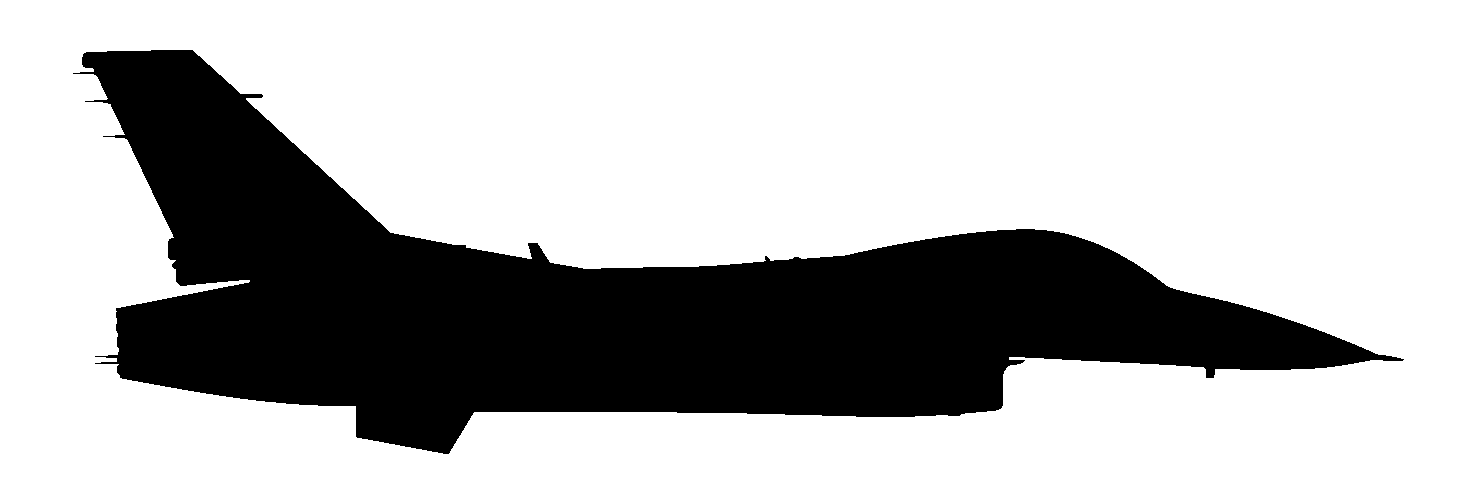
\includegraphics[
                    width=7.5mm,
                ]{diagrams/aircraft/silhouette_f16_side.pdf}
            };
    
            % approach
            \draw[->]
            (high_key)
            .. controls ($(high_key)+(-10:20)$) and ($(low_key)+(10:20)$) ..
            (low_key);
            \draw[->]
            (low_key)
            .. controls ($(low_key)+(190:10)$) and ($(base_key)+(70:1)$) ..
            (base_key);
            \draw[->]
            (base_key)
            .. controls ($(base_key)+(-60:5)$) and ($(td_des)+(177:5)$) ..
            (td_des);

            \node[red, font=\small\bfseries, above] at (high_key) {A};
            \node[red, font=\small\bfseries, above] at (low_key) {B};
            \node[red, font=\small\bfseries, left] at (base_key) {C};
            \node[red, font=\small\bfseries, below] at (td_des) {D};
    
            \filldraw[red] (high_key) circle (2pt);
            \filldraw[red] (low_key) circle (2pt);
            \filldraw[red] (base_key) circle (2pt);
            \filldraw[red] (td_des) circle (2pt);
        \end{tikzpicture}
        \caption{side view}
    \end{subfigure}
    \begin{subfigure}[t]{\linewidth}
        \centering
        \begin{tikzpicture}[figstyle]

            % coordinates
            \coordinate (td_des) at (0,0);
            \coordinate (high_key) at (10,0);

            % runway
            \draw[thick]
            ($(td_des)+(-5,-2)$) 
            -- ($(td_des)+(-5,2)$) 
            -- ($(td_des)+(30,2)$) 
            -- ($(td_des)+(30,-2)$) 
            -- cycle;
            \draw[thick]
            ($(td_des)+(-1,-1.33)$) -- ($(td_des)+(1,-1.33)$)
            ($(td_des)+(-1,-0.66)$) -- ($(td_des)+(1,-0.66)$)
            ($(td_des)+(-1,0.66)$) -- ($(td_des)+(1,0.66)$)
            ($(td_des)+(-1,1.33)$) -- ($(td_des)+(1,1.33)$);

            \draw[->]
            (high_key) 
            arc (90:-90:12)
            -- ++(-20,0) node (low_key) {};
            \draw[->]
            (low_key)
            arc(270:180:12) node (base_key) {};
            \draw[->]
            (base_key)
            arc (180:90:12)
            -- (td_des);

            \node[red, font=\small\bfseries, above=2mm] at (high_key) {A};
            \node[red, font=\small\bfseries, below] at (low_key) {B};
            \node[red, font=\small\bfseries, left] at (base_key) {C};
            \node[red, font=\small\bfseries, above=2mm] at (td_des) {D};

            \draw[<->, thin] (high_key) -- ++(0,-24) node[font=\small, pos=0.5] {1 nm};
            \draw[<->, thin] (base_key) -- (td_des) node[font=\small, pos=0.5, below right] {1.25 nm};

            \filldraw[red] (high_key) circle (2pt);
            \filldraw[red] (low_key) circle (2pt);
            \filldraw[red] (base_key) circle (2pt);
            \filldraw[red] (td_des) circle (2pt);
        \end{tikzpicture}
        \caption{top-down view}
    \end{subfigure}
    \caption{Flameout landing pattern --- Overhead Approach}
    \label{fig:proc_basic:landing:overhead2}
\end{figure}

\subsubsection{STRAIGHT-IN APPROACH}

\marginfigeometry

\subsubsection{PROCEDURE}

\begin{checklistenumerate}
    \blueitem[Stores]\dotfill Jettison (if required)
    \blueitem[Airspeed]\dotfill 200 kts
    \begin{itemize}
        \item increase speed 5 kts every 1000 lbs of fuel/stores
    \end{itemize}
    \blueitem[EPU]\dotfill \textbf{ON}
    \blueitem[JFS Switch]\dotfill \textbf{START 2}
    \blueitem[AIR SOURCE Knob]\dotfill \textbf{RAM}\\
    \hfill(below 25'000 ft MSL)
    \blueitem[LG Handle]\dotfill \textbf{DN}
    \blueitem[ALT GEAR Handle]\dotfill Pull\\
    \hfill(if required)
    \blueitem[Airspeed]\dotfill 190 kts in pattern
    \blueitem[DRAG CHUTE Switch]\dotfill \textbf{DEPLOY}\\
    \hfill(if required)
    \blueitem[HOOK Switch]\dotfill DN\\
    \hfill(if required)
\end{checklistenumerate}

\clearpage

\marginfigrestore